%%\documentclass[a4paper, 12pt]{scrreprt}

\documentclass[a4paper, 12pt]{scrartcl}
%usepackage[german]{babel}
\usepackage{microtype}
%\usepackage{amsmath}
%usepackage{color}
\usepackage[utf8]{inputenc}
\usepackage[T1]{fontenc}
\usepackage{wrapfig}
\usepackage{lipsum}% Dummy-Text
\usepackage{multicol}
\usepackage{alltt}
%%%%%%%%%%%%bis hierhin alle nötigen userpackage
\usepackage{tabularx}
\usepackage[utf8]{inputenc}
\usepackage{amsmath}
\usepackage{amsfonts}
\usepackage{amssymb}

%\usepackage{wrapfig}
\usepackage[ngerman]{babel}
\usepackage[left=25mm,top=25mm,right=25mm,bottom=25mm]{geometry}
%\usepackage{floatrow}
\setlength{\parindent}{0em}
\usepackage[font=footnotesize,labelfont=bf]{caption}
\numberwithin{figure}{section}
\numberwithin{table}{section}
\usepackage{subcaption}
\usepackage{float}
\usepackage{url}
%\usepackage{fancyhdr}
\usepackage{array}
\usepackage{geometry}
%\usepackage[nottoc,numbib]{tocbibind}
\usepackage[pdfpagelabels=true]{hyperref}
\usepackage[font=footnotesize,labelfont=bf]{caption}
\usepackage[T1]{fontenc}
\usepackage {palatino}
%\usepackage[numbers,super]{natbib}
%\usepackage{textcomp}
\usepackage[version=4]{mhchem}
\usepackage{subcaption}
\captionsetup{format=plain}
\usepackage[nomessages]{fp}
\usepackage{siunitx}
\sisetup{exponent-product = \cdot, output-product = \cdot}
\usepackage{hyperref}
\usepackage{longtable}
\newcolumntype{L}[1]{>{\raggedright\arraybackslash}p{#1}} % linksbündig mit Breitenangabe
\newcolumntype{C}[1]{>{\centering\arraybackslash}p{#1}} % zentriert mit Breitenangabe
\newcolumntype{R}[1]{>{\raggedleft\arraybackslash}p{#1}} % rechtsbündig mit Breitenangabe
\usepackage{booktabs}
\renewcommand*{\doublerulesep}{1ex}
\usepackage{graphicx}



%\begin{document}

\section{Theoretische Grundlagen}
Die Quantisierung der energetischen Zustände eines Moleküls lassen sich in Abhängigkeit von dem benötigten Energiebetrag $E = h \cdot \nu$ zu einer diskreten Anregung verstehen. So entspricht zum Beispiel die benötigte Energie, um ein rotatorisch angeregten Zustand zu induzieren, dem Bereich der Mikrowellenstrahlung, also dem Frequenzbereich von 0.5-100 GHz (abhängig vom betrachteten Molekül). Schwingungsniveaus benötigen hingegen höherenergetische Strahlung um im Allgemeinen angeregt zu werden, also elektromagnetische Wellen im infraroten Spektralbereich. Die elektronische Anregung eines Moleküls benötigt die größte Energiemenge und liegt im Bereich von 1 bis 10eV, was einem Wellenlängenintervall von ungefähr 125 nm bis 1250 nm entspricht. Es ist somit ersichtlich, dass die elektronische Anregung zum großen Teil im Bereich des sichtbaren Lichtes stattfindet, für das menschliche Auge somit wahrzunehmen ist. Da das menschliche Auge jedoch kein gutes Spektrometer ist, bedienen sich physikalische Chemiker in der heutigen Zeit an digitalen Messeinheiten um z.B die elektronische Anregung eines Moleküls zu beobachten.\\
\\
Bei dem Verbrennungsprozess von kurzkettigen Kohlenwasserstoffen enstehen neben $OH$ und $CH$ insbesondere $C_2$ Radikale, die für die blaue Farbe der rauschenden Flamme des Bunsenbrenners verantwortlich sind. Die allgemein bekannte rotgelbe Farbe der Flamme einer Verbrennung entsteht aus Absorptionseffekten der bei der Verbrennung entstehenden Rußpartike, wobei die rauschende Flamme durch ausreichende Sauerstoffzufuhr die Rußbildung unterbindet. Durch den Verbrennungsprozess entstehen neben $C_2$ Radikale im Grundzustand ebenfalls solche, die sich im elektronisch angeregten Zustand befinden. Ferner liegen in allen populierten elektronischen Zuständen ebenfalls eine Vielzahl von Schwingugnszuständen vor. Die unterschiedlichen Relaxationen der energetisch höher liegenden Elektronischen Zustände in den Grundzustand  induziert ein Photoemissionsspektrum, welches für das $C_2$ Radikal als \textit{Swan Banden} beschrieben wird. Beschränken wir uns auf den relevanten elektronischen Übergang als $d(^3\Pi_g) \rightarrow a(^3\Pi_u)$. Basierend auf der großen Anzahl ebenfalls populierter Schwingungsniveaus in den elektronischen Zuständen resultiert eine Vielzahl von möglichen Übergängen durch Photoemissionen zwischen Schwingungsniveaus im elektronisch angeregten Zustand in den Grundzustand. Unter Annahme keiner großen geometrischen Änderung des $C_2$ Radikals durch die elektronische Anregung folgt die ungefähre Äquidistanz der Schwingungsniveaus bezogen auf die beiden betrachteten elektronischen Zustände. Ferner, dass ebenfalls die Progressionen für diskrete $\Delta \nu$ Werte vorliegen, da die Energiedifferenzen sehr ähnlich sind. Es bilden sich also Sequenzen gemäß Abbildung \ref{Bandensystem}. Alle Sequenzen ergeben das \textit{Bandensystem} zwischen den beiden elektronischen Zuständen, welches durch folgende Gleichung beschrieben werden kann: 
\begin{equation}
\nu = \nu_e + \omega_e'(v'+\frac{1}{2}) - \omega_e'x_e'(v'+\frac{1}{2})^2 - [\omega_e'' (\nu''+\frac{1}{2})-\omega_e''x_e''(\nu''+\frac{1}{2})^2]
\end{equation}
wobei die bekannten Größen der Wellenzahl des Übergangs als $\nu$, die Schwingungsquantenzahlen bezogen auf die elektronsichen Zustände $\nu',\nu''$, die Schwingungskonstanten $\omega_e',\omega_e''$ sowie die Anharmonizitätskonsten $\omega_e'x_e',\omega_ex_e''$ verwendet wurden. Ebenfalls wird die gängige Notation mit zwei $''
$ für den Grundzustand benutzt. 
\begin{figure}[H]
	\centering	
	\begin{minipage}{0.6\textwidth}
		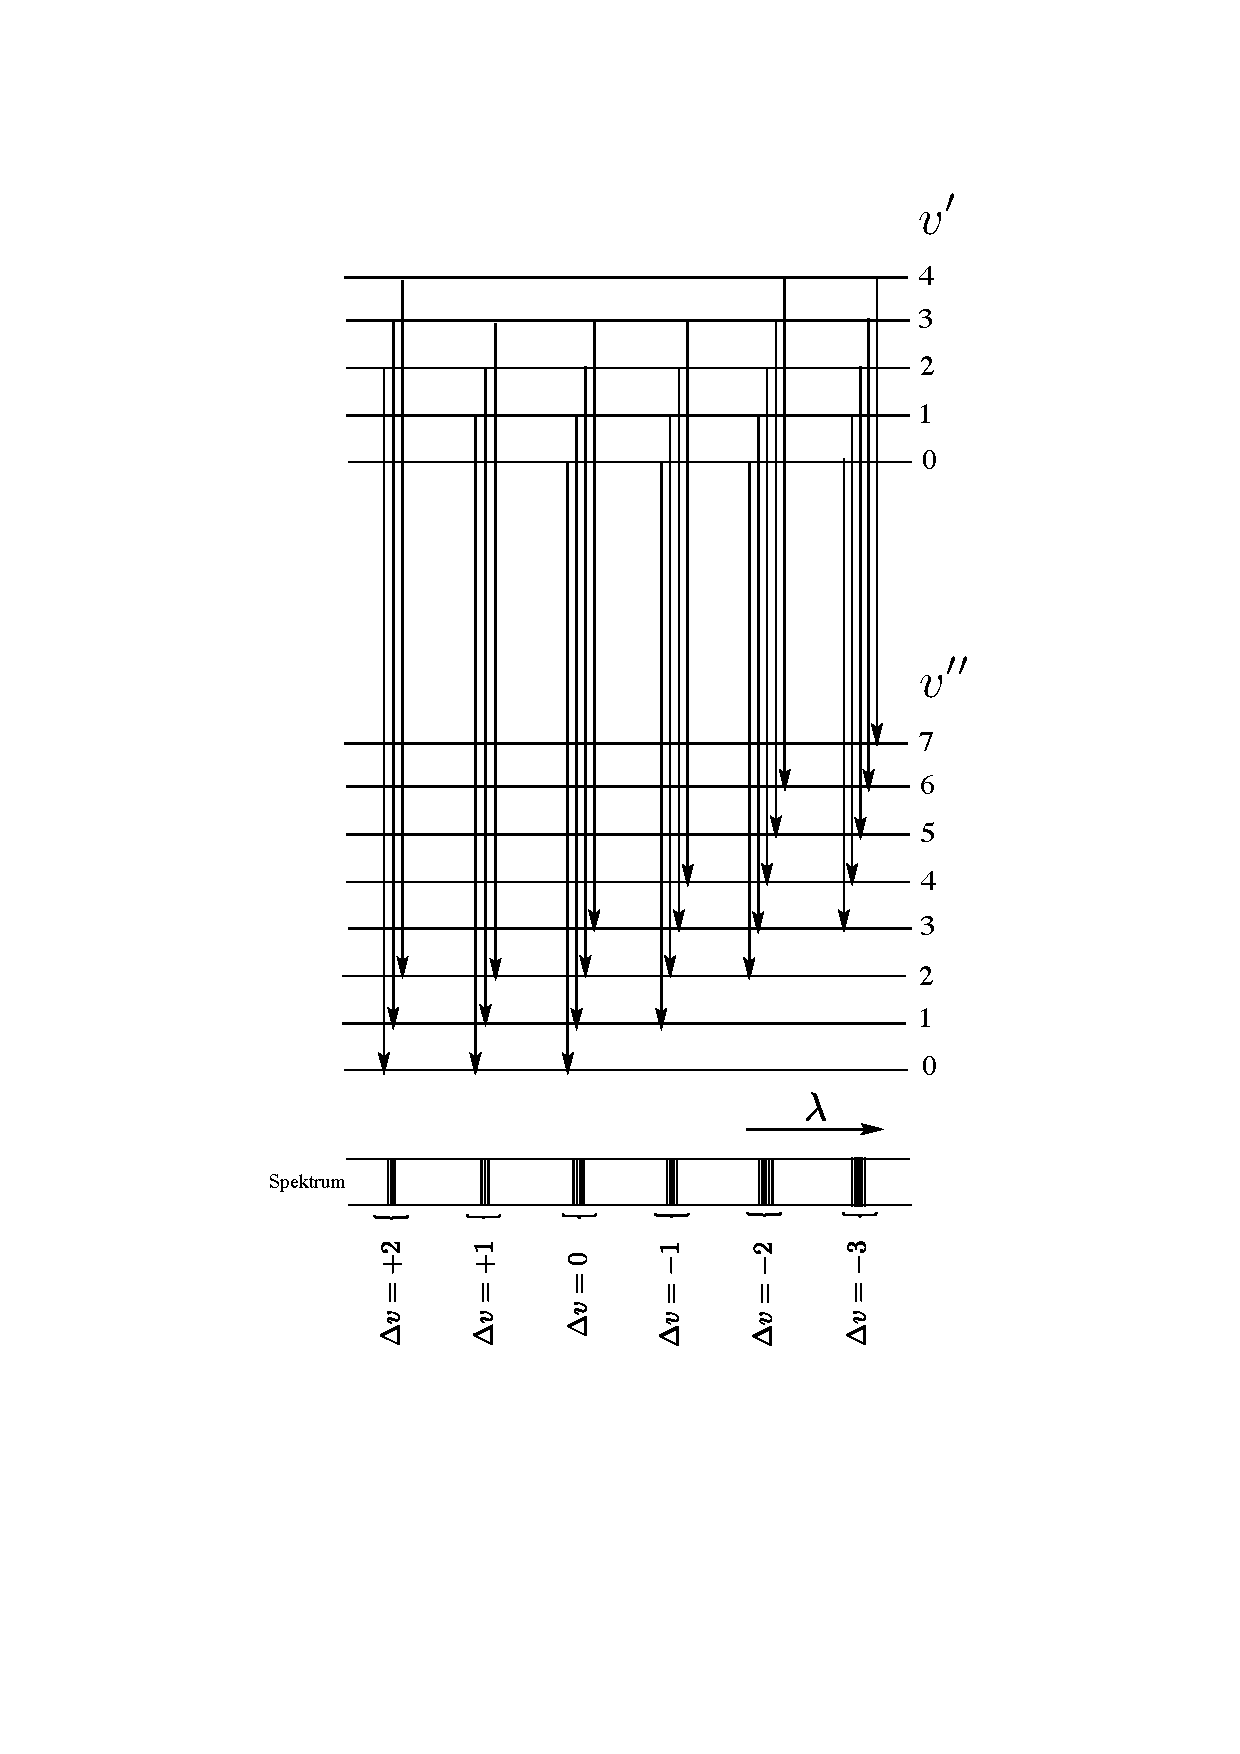
\includegraphics[width=\columnwidth]{Bilder/Bandensysteme.pdf}
		\caption{Energieniveau-Diagramm zur Darstellung der Sequenzen (Diagonalgruppen) in einem Bandensystem}
		\label{Bandensystem}
	\end{minipage}
\end{figure}

%%%
%
%
%
% Hier kommt Abbildung 1 hin die ich aber noch anfertige.
%
%
%%%
%\end{document}